\documentclass{article}
\usepackage{tabularx}
\usepackage{graphicx} 
\usepackage[utf8]{inputenc}
\usepackage[T1]{fontenc}
\usepackage[polish]{babel}
\usepackage{adjustbox}

\title{Sumowanie szeregów numerycznych}
\author{Hubert Kowalski}
\date{March 2023}

\begin{document}

\maketitle

\section{Wstęp}

Celem projektu jest zbadanie zachowania liczb zmiennoprzecinkowych w środowisku języków programowania. W moim przypadku został użyty język Java.

\section{Hipotezy}


\begin{itemize}
\item H1: Sumowanie od końca daje dokładniejsze wyniki niż sumowanie od początku
\item H2: Używając rozwinięcia wokół 0 (szereg MacLaurina), przy tej samej liczbie składników szeregu dokładniejsze wyniki uzyskujemy dla małych argumentów
\item H3: Sumowanie elementów obliczanych na podstawie poprzedniego daje dokładniejsze wyniki niż obliczanych bezpośrednio ze wzoru
\end{itemize}

Oraz odpowiedzieć na pytanie:

Q1: Jak zależy dokładność obliczeń (błąd) od liczby składników?

\section{Metoda}

Badanie zachowania zostało wykonane w spósób sformułowania czterech sposobów obliczania przybliżenia funkcji cosinus przy pomocy sumowania 20 elementów szeregów potęgowych. 
Wzór na sam szereg potęgowy wygląda następująco: 

\begin{center}
\begin{math}
\cos(x) = \sum_{n=0}^{\infty} \frac{(-1)^n}{(2n)!} x^{2n}
\end{math}
\end{center}

\clearpage

\subsection{Sposoby}

Badanie zostało wykonane na cztery sposoby:

\begin{itemize}
\item V1 (t\_cos) Sumując elementy szeregu potęgowego obliczane bezpośrednio ze wzoru Taylora w kolejności od początku
\item V2 (t\_cos\_rev) Sumując elementy szeregu potęgowego obliczane bezpośrednio ze wzoru Taylora w kolejności od końca
\item V3 (power\_series\_cos) Sumując elementy szeregu potęgowego od początku ale obliczając kolejny wyraz szeregu na podstawie poprzedniego
\item V4 (power\_series\_cos\_rev) Sumując elementy szeregu potęgowego od początku ale obliczając kolejny wyraz szeregu na podstawie końca
\end{itemize}

\subsection{Błędy absolutne}

Błędy absolutne zostały wyliczone na podstawie funkcji cos z biblioteki Math Javy. Dodatkowo obliczenia zostały wykonane dla 1 000 000 próbek.

\centerline{Wykres błędów absolutnych ma się następująco:}

\hspace{0.5cm}

\centerline{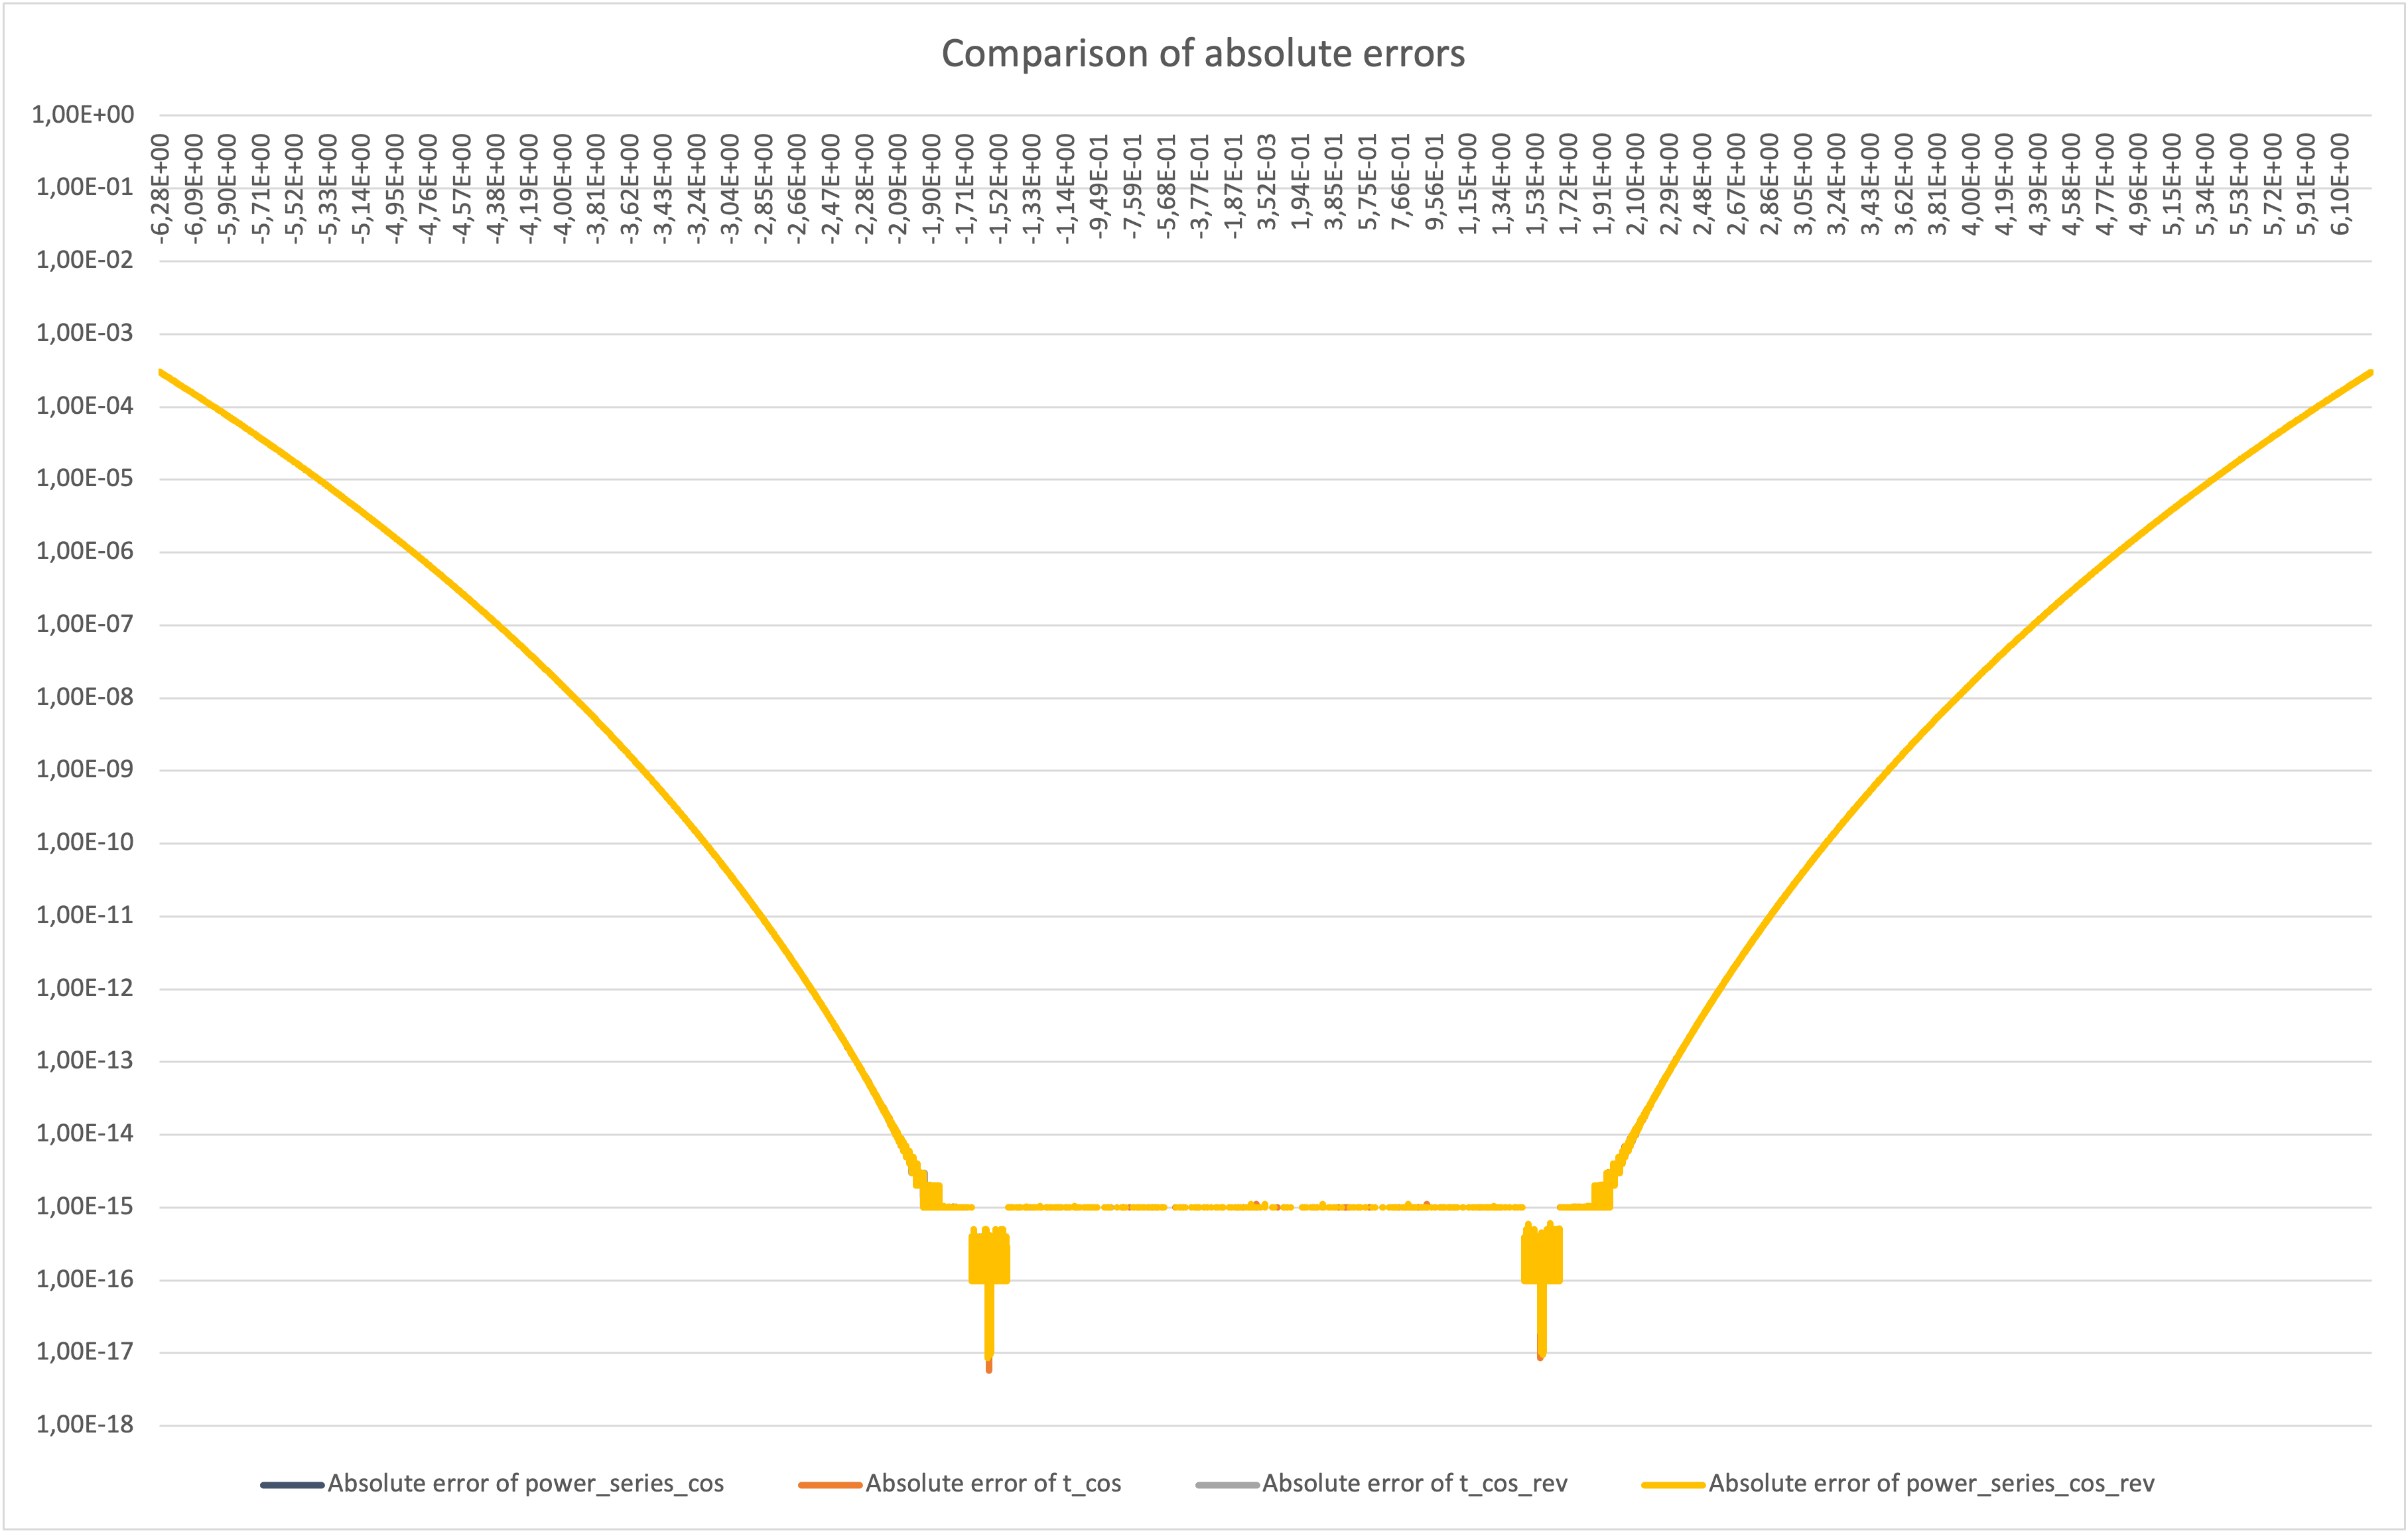
\includegraphics[scale=0.50]{comparison.png}}

\hspace{0.5cm}

Wykres został przeskalowany logarytmicznie, żeby uwydatnić błędy, które znajdowały się przy brzegach zakresu \begin{math}[-2\pi; 2\pi]\end{math} maksymalny błąd jaki popełniają wszystkie funkcje to ok. 1,00E-03.

\clearpage

Porównanie średnich błędów absolutnych ma się następująco:

\hspace{0.5cm}

\centerline{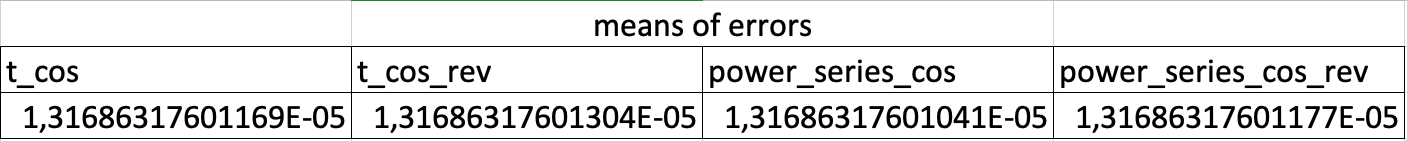
\includegraphics[scale=0.3]{means.png}}

\subsection{Odpowiedzi na hipotezy}

Dzięki tym danym jestem w stanie odpowiedzieć na podane hipotezy

\subsection{H1}

Odpowiedź: Hipoteza ta jest fałszywa, ponieważ średnia błędu absolutnego t\_cos\_rev jest o 1,35356E-17 większa od t\_cos, analogicznie średnia power\_series\_rev jest o 1,36321E-17 większa od power\_series\_cos\_rev.

\subsection{H2}

Odpowiedź: Jest to prawda patrząc na wykres jesteśmy w stanie to stwierdzić, ponieważ wykres błędu absolutengo w okół zera daje wartości bliższe zeru niż na skrajach przedziału.

\subsection{H3}

Odpowiedź: Tak, to prawda. Średnia błędu absolutnego power\_series\_cos jest o 1,28088E-17 mniejsza od błędu t\_cos, analogicznie sumując je od końca różnica wynosi 1,27123E-17.

\subsection{Q1}

\begin{center}
    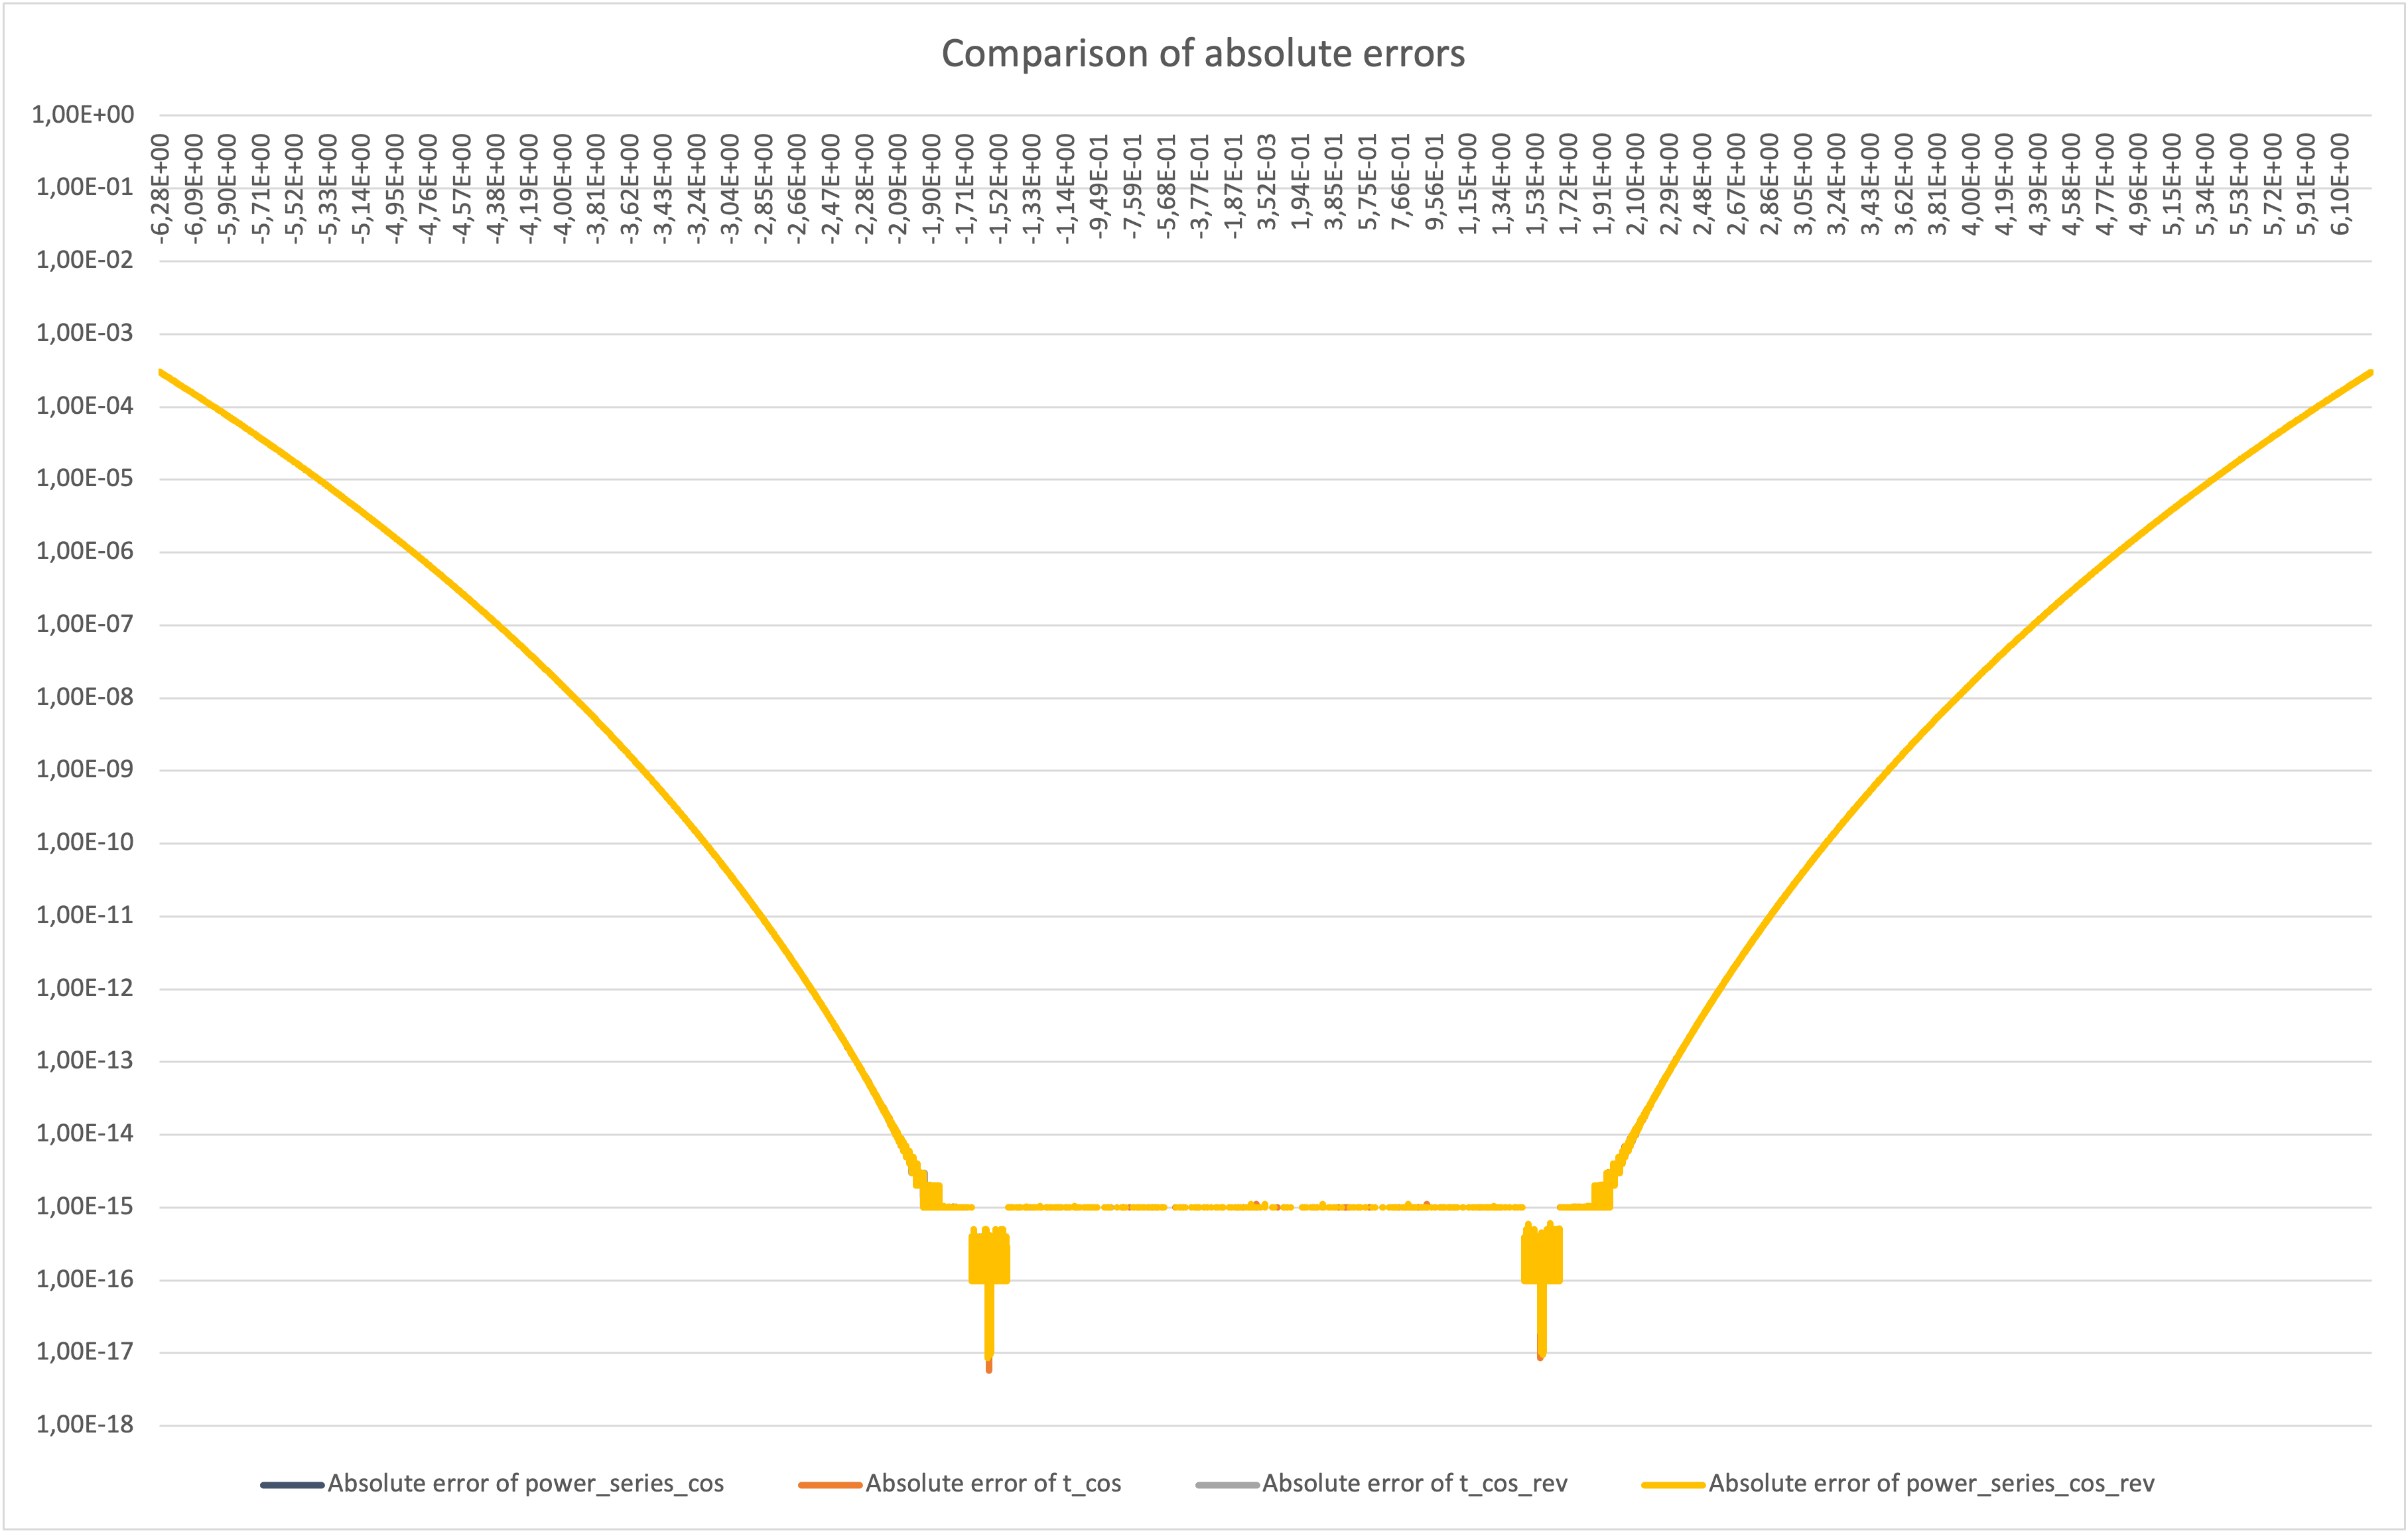
\includegraphics[scale=0.45]{comparison.png}
    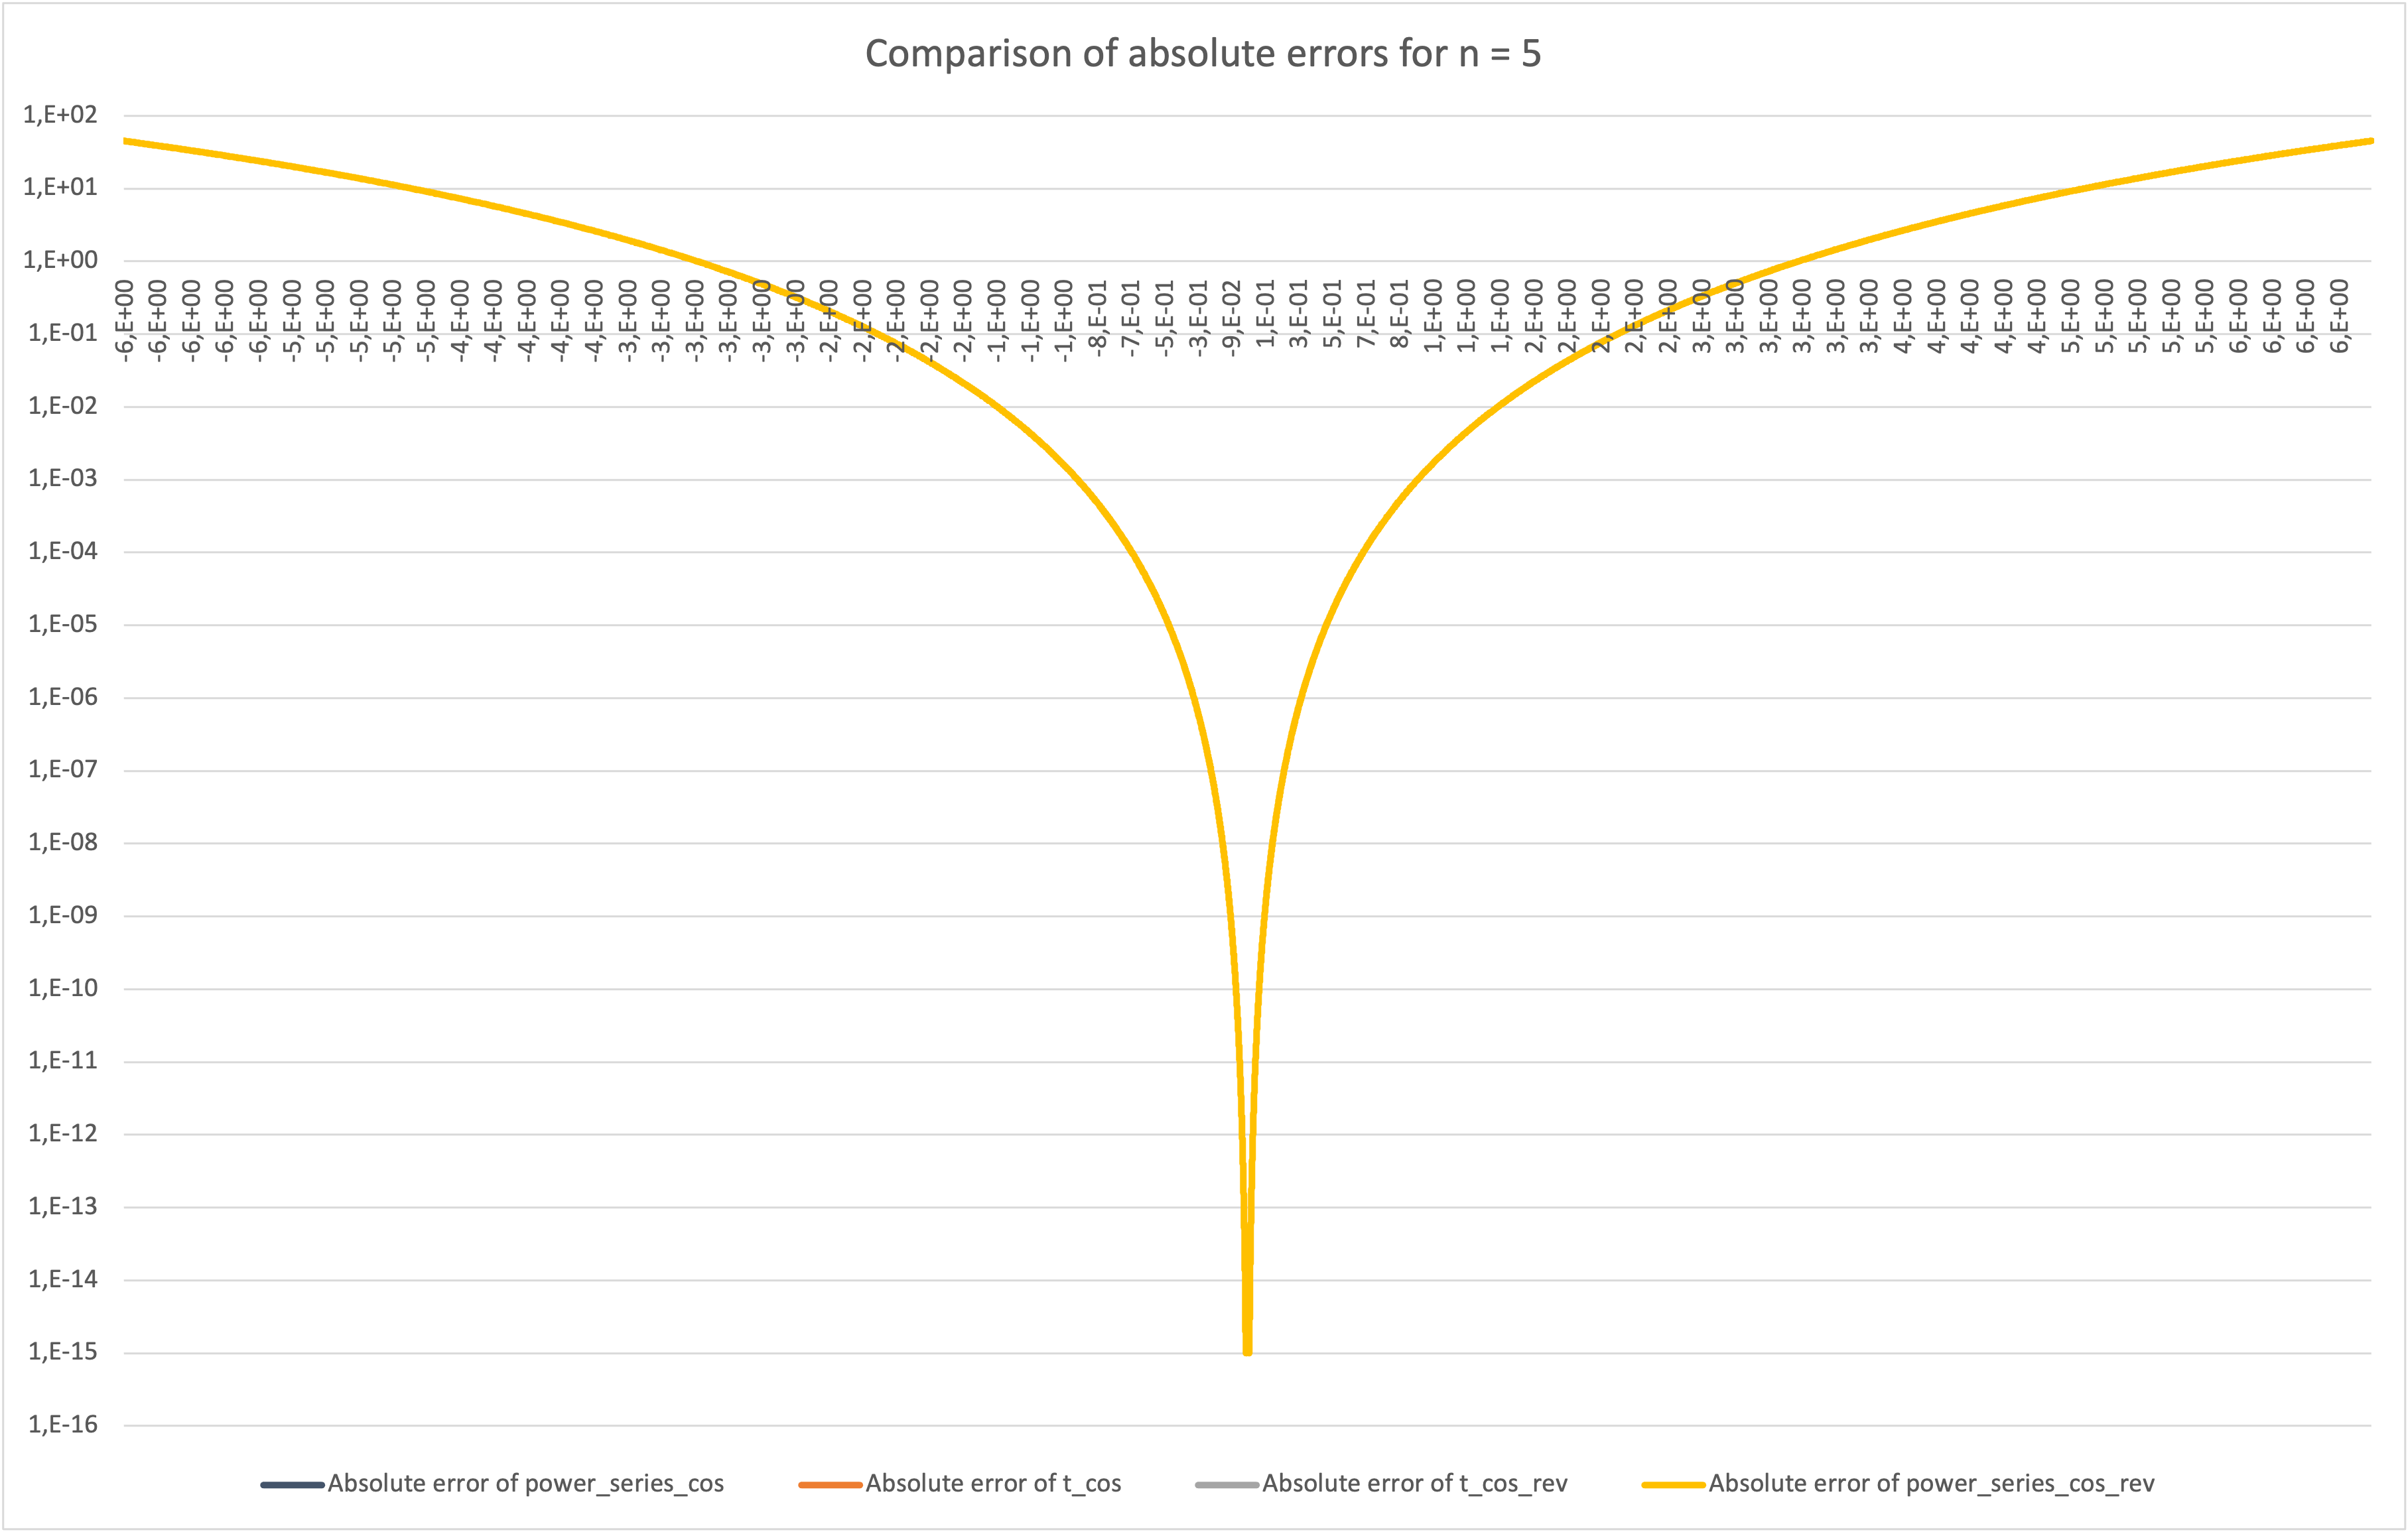
\includegraphics[scale=0.45]{comparison-n5.png} \\
    \textit{Porównanie wykresów błędów dla $n = 20$ i $n = 5$}
\end{center}

Odpowiedź: Błąd jest tym mniejszy im więcej sumujemy składników szeregu. Wynika to z samego twierdzenia Taylora oraz sami możemy to zauważyć zwiększając ilość elementów sumy w samym skrypcie.

\end{document}
